\begin{answer}
    
    The fitted lines seem to fit much better straightaway from $k=0$ onwards, due to the existence of the sine mapping of x. At k=20, we can even see overfitting with the model being more sensitive to specific points and not generalizing anymore as well, whereas the other lines basically seem on top of each other.

    After checking the learned parameters for different $k$, it also seems like the other features are $10^1$ to $10^3$ times smaller and on an absolute level negligibly small.

    \begin{figure}[h]
        \centering
        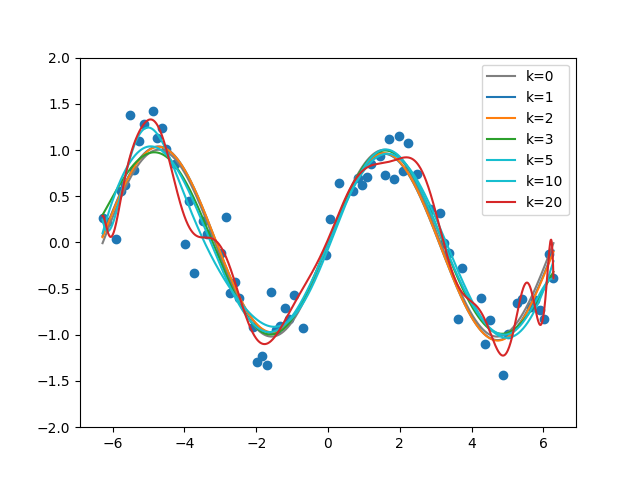
\includegraphics[width=0.8\textwidth]{src/featuremaps/plot-sine-degrees[0, 1, 2, 3, 5, 10, 20].png}
        \caption{Polynomial regression with sine features}
        \label{fig:sine-features}
    \end{figure}
\end{answer}
